\documentclass[10pt, conference, compsocconf]{IEEEtran}
\usepackage[hidelinks]{hyperref}
\usepackage{graphicx}
\usepackage{color}
\usepackage{float}
\newcommand\todo[1]{\textbf{\textcolor{red}{#1}}}
\DeclareGraphicsExtensions{.pdf,.jpeg,.png}
\usepackage[round]{natbib}
\usepackage{tabularx}
\hyphenation{op-tical net-works semi-conduc-tor}
\usepackage[linesnumbered]{algorithm2e}
\usepackage{listings}
\usepackage{xcolor}
%\usepackage{caption}

\colorlet{punct}{red!60!black}
\definecolor{background}{HTML}{EEEEEE}
\definecolor{delim}{RGB}{20,105,176}
\colorlet{numb}{magenta!60!black}

\lstdefinelanguage{json}{
    basicstyle=\normalfont\ttfamily,
    numbers=left,
    numberstyle=\scriptsize,
    stepnumber=1,
    numbersep=8pt,
    showstringspaces=false,
    breaklines=true,
    frame=lines,
    backgroundcolor=\color{background},
    literate=
     *{0}{{{\color{numb}0}}}{1}
      {1}{{{\color{numb}1}}}{1}
      {2}{{{\color{numb}2}}}{1}
      {3}{{{\color{numb}3}}}{1}
      {4}{{{\color{numb}4}}}{1}
      {5}{{{\color{numb}5}}}{1}
      {6}{{{\color{numb}6}}}{1}
      {7}{{{\color{numb}7}}}{1}
      {8}{{{\color{numb}8}}}{1}
      {9}{{{\color{numb}9}}}{1}
      {:}{{{\color{punct}{:}}}}{1}
      {,}{{{\color{punct}{,}}}}{1}
      {\{}{{{\color{delim}{\{}}}}{1}
      {\}}{{{\color{delim}{\}}}}}{1}
      {[}{{{\color{delim}{[}}}}{1}
      {]}{{{\color{delim}{]}}}}{1},
}

\begin{document}
\title{Biclustering using Biological Context Information}


\author{\IEEEauthorblockN{Willi Gierke}
\IEEEauthorblockA{
Hasso Plattner Institute\\
Potsdam, Germany\\
willi.gierke@student.hpi.de}
}

\maketitle

\begin{abstract}
Recently, RNA sequencing has become the crucial technique to obtain gene expression data.
Biclustering has emerged as a powerful tool to find genes with similar expression patterns under specific conditions in this data.
However, most approaches are limited as they only rely on patterns that can be found in the data itself.
This prevents them from uncovering biological processes that do not manifest in the chosen dataset.

We propose an algorithm that extends biclustering by including additional biological context information.
The presented algorithm is evaluated on a public cancer data set, yielding promising results by finding new patterns and suggesting encouraging possibilities for further research.
\end{abstract}

\begin{IEEEkeywords}
biclustering; pathway

\end{IEEEkeywords}

\IEEEpeerreviewmaketitle


\section{Introduction}
\label{sec:introduction}
With recent advances in sequencing technology, RNA sequencing has become the tool of choice to obtain gene expression data.
In comparison to the traditional microarray technology, it yields a higher specificity and sensitivity and it supports detecting weakly expressed genes as well \citep{Zhao14}.
This allows to also study weakly expressed genes whose functions can then be inferred.
The underlying assumption is that genes sharing similar expression patterns also contribute to similar biological processes.

An approach to group genes into collections of akin patterns is clustering.
The corresponding algorithms make it possible to discover disease-specific genes.
However, studies have shown that a gene contributes to ten different biological processes on average, which cannot be reflected by traditional clustering approaches as they assign each gene to a single cluster only.
Therefore, single clustering algorithms are not suitable to capture this property.
In contrast, biclustering approaches assign genes and samples to multiple clusters.
Their main advantage is that they support finding overlapping clusters, a characteristic that reflects
the behavior of genes very well. They also simultaneously assign both genes and samples to
clusters. This allows interpreting genes of a cluster as contributors to biological processes
that are shared across a specific set of samples only.
However, most biclustering approaches are limited as they only rely on patterns that can be found in the data itself.
Hidden biological processes that are not represented by the sampled data can not be discovered.
Moreover, the algorithms can find structures that are not of interest.
Due to their strong dependence on the given data set, they can also detect nonexistent patterns that simply result from noise or by accident.
Including biological context information can support the algorithm in finding patterns that contribute to the same processes.
By adjusting the added context information, we can regularize the algorithm to find structures that are of interest only.
The results of such analyses can highly improve the plausibility of the found patterns since they no more
only depend on statistical properties of the expression data alone.

We model the problem of finding biclusters as a graph problem while incorporating third-party data from the biological database STRING by adding corresponding edges and searching for maximal cliques.

In this work, we propose an approach that extends the biclustering algorithm \textit{BiMax} by including additional biological context information.
The remainder of this paper is structured as follows.
Section \ref{sec:related} describes related literature discussing the targeted problem.
In Section \ref{sec:algorithm} we present the proposed algorithm.
Next, Section \ref{sec:evaluation} evaluates our approach on a public cancer data set.
Section \ref{sec:discussion} discusses advantages and limitations of the algorithm.
Lastly, Section \ref{sec:conclusion} concludes this paper.


\section{Related Work}
\label{sec:related}
\cite{Ponzoni2014} demonstrate how to combine gene expression data with pathway information to infer association rules between the pathways.
For each pathway, they generate a matrix containing expression data of the genes that are involved in the pathway.
Lastly, they reduce the matrices using principal component analysis and apply association rule mining to detect relationships between the pathways.
While this approach successfully demonstrates how to combine context information with gene expression data, it does not aim at improving biclustering of the mentioned data.
\cite{Dutta2012} present an approach that uses both gene expression data and information from neighboring pathways to detect dependencies and relations between pathways.
\cite{Liu2012} use gene expression data, protein-protein interactions and cellular pathways to infer dysregulated pathways.

Adding third-party data has also shown great improvements in tasks for single-mode clustering.
As presented by \cite{Hindle11}, incorporating meta information of videos enabled the clustering algorithm to greatly improve the quality of video clusters.


\cite{Prelic06} present \textit{Bimax}, a divide-and-conquer algorithm that expects a binary expression matrix.
It recursively divides the input matrix into possibly overlapping submatrices until all inclusion-maximal biclusters are found.
As shown by \cite{Voggenreiter12}, \textit{Bimax} can be reformulated as a graph problem.
In this setting, a bipartite graph is built between a set of samples and a set of genes.
A connection between two nodes of the different sets is drawn if the gene is significantly expressed in the corresponding sample.
Finding all inclusion-maximal biclusters is then equal to finding all maximal bicliques in the bipartite graph.
This objective can for example be achieved by using the Bron-Kerbosch algorithm \citep{Bron73}.

\section{Algorithm}
\label{sec:algorithm}
In this section we elaborate on the algorithm steps.
First, we present the preprocessing steps that are necessary.
Next, we explain how the bipartite graph is built based on the input.
We then elaborate on in which way context information is added.
Lastly, we show how biclusters can be found.

% Our algorithm incorporates biological context information while finding biclusters of genes and samples.
% It expects a normalized gene expression matrix as input.
% The matrix will be binarized with respect to the hyperparameter $\tau_e$.
% Based on that, a unweighted bipartite graph between samples and genes is built.
% Depending on the second hyperparameter $\tau_i$, additional edges between gene nodes are drawn that introduce biological context information.
% Lastly, overlapping biclusters can be found by using the Bron-Kerbosch algorithm that searches for maximal cliques in the graph.

\subsection{Preprocessing}
\label{sec:preprocessing}
% \begin{figure}[h]
% \centering
% 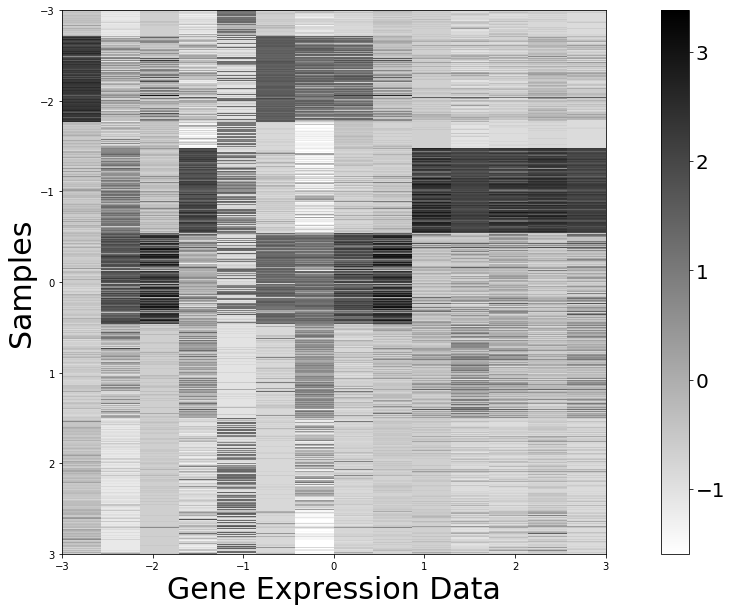
\includegraphics[width=2.5in]{figures/bicluster_weighted.png}
% \caption{Log-Normalized Gene Expression Matrix. The darker a cell, the higher the corresponding gene is expressed in the related sample.}
% \label{fig:bicluster_weighted}
% \end{figure}

% \begin{table}[h]
%     \centering
%     \begin{tabular}{r|c|c|c}
%         Sample/Gene & G$_1$ & ... & G$_n$ \\ \hline
%         S$_1$	        & 0.2546451 & ... & -0.390651\\
%         ...	        & ... & ... & ...\\
%         S$_m$	        & -1.294704 & ... & 0.044671\\
%     \end{tabular}
%     \caption{Example of a $m{\times}n$ Gene Expression Matrix. A high value means high expression of the gene in the corresponding sample.}
%     \label{tab:weighted}
% \end{table}

\begin{table}
\centering
    \begin{tabular}{r|c|c|c}
         & G$_1$ & ... & G$_n$ \\ \hline
        S$_1$	        & 0.2546451 & ... & -0.390651\\
        ...	        & ... & ... & ...\\
        S$_m$	        & -1.294704 & ... & 0.044671\\
    \end{tabular}
    $\Rightarrow$
    \begin{tabular}{r|c|c|c}
         & G$_1$ & ... & G$_n$ \\ \hline
        S$_1$	        & 1 & ... & 0\\
        ...	        & ... & ... & ...\\
        S$_m$	        & 0 & ... & 1\\
    \end{tabular}
    \caption{Binarization of a Gene Expression Matrix with $m$ Samples and $n$ Genes Using a Threshold of $\tau_e=0$.}
    \label{tab:binarization}
\end{table}

First, logarithmic scaling is applied since the magnitudes of the gene expression levels are not of interest.
It is only desirable to compare whether a gene is over- or underregulated regarding various samples.
Therefore, binarizing the matrix with respect to an expression threshold $\tau_e$ is in accordance with this objective.
$\tau_e$ can be set to the mean or median of each gene expression level over all samples.
This is also necessary because the algorithm that finds biclusters only works on undirected, unweighted graphs.
Since the gene expression matrix functions as the graph's adjacency matrix, the matrix is supposed to be binary.
In this matrix a cell is set to one if the corresponding gene is higher expressed in the sample than in one half of the remaining samples.
Table \ref{tab:binarization} shows the binarization of a gene expression matrix when setting $\tau_e=0$.
% To also build clusters for genes that are underregulated, in an other experiment the cell can simply be set to one if the corresponding expression is below average.
% \begin{table}[h]
%     \centering
%     \begin{tabular}{r|c|c|c}
%         Sample/Gene & G$_1$ & ... & G$_n$ \\ \hline
%         S$_1$	        & 1 & ... & 0\\
%         ...	        & ... & ... & ...\\
%         S$_m$	        & 0 & ... & 1\\
%     \end{tabular}
%     \caption{Example of a Binarized $m{\times}n$ Gene Expression Matrix}
%     \label{tab:binarized}
% \end{table}
% \begin{figure}[h]
% \centering
% 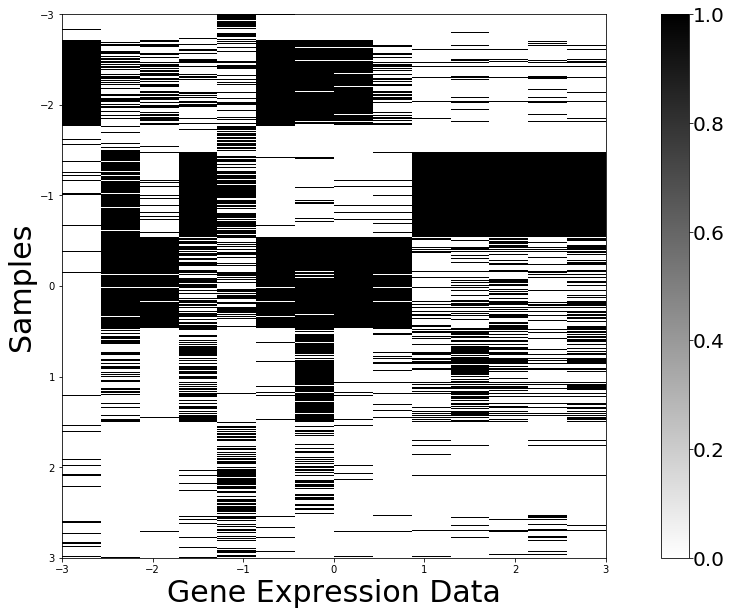
\includegraphics[width=2.5in]{figures/bicluster_binarized.png}
% \caption{Binarized Gene Expression Matrix. Gene expressions that exceed a threshold $\tau_e$ are set to one (black) and zero (white) otherwise.}
% \label{fig:bicluster_binarized}
% \end{figure}
\subsection{Graph Building}
Based on this matrix a bipartite graph is built.
A bipartite graph is a triple $G=(V, U, E)$ where $V$ and $U$ are disjoint sets of vertices.
$E$ is the set of edges that connects vertices from $V$ with vertices from $U$.
In this instance, $V$ corresponds to the samples and $U$ to the genes.
An edge between a sample and a gene is drawn if the corresponding cell in the matrix equals one.
Formally, let $A$ be the given gene expression matrix.
$A_{ij}$ corresponds to the expression of gene $j$ in sample $i$.
It holds that:

\begin{equation}
    A_{ij} > \tau_e \iff (i, j) \in E
\end{equation}

In order to incorporate biological context information, an edge is drawn between two nodes of the set of genes if both genes are known to interact with each other.
This context information can be the certainty of a third-party data source that two genes interact with each other.
This is for example the case if genes contribute so the same pathways.
The edge is drawn if the confidence score of the third-party source is above a threshold $\tau_i$.
Let $s_\alpha(x, y)$ be a score function that returns the confidence that the genes $x$ and $y$ interact with each other based on data from $\alpha$.
Furthermore, let $g_1, g_2 \in U$.
It holds that:

\begin{equation}
    s_\alpha(g_1, g_2) > \tau_i \iff (g_1, g_2) \in E
\end{equation}

By choosing the external data source and the interaction criterion $\alpha$, the algorithm can be pushed to focus on expression patterns of the desired domain.
In Subsection \ref{subsec:implementation} we elaborate on how to define the score using data from the biological database STRING \citep{StringDB15}.

\subsection{Finding Biclusters}
Based on the resulting graph, we are identifying biclusters by finding the maximal cliques in the graph.
A clique is a set of vertices such that each vertex is directly connected to each other of the clique.
Thus, the subgraph that is induced by a clique is fully-connected.
A maximal clique is a clique that can not be extended by more nodes.
The Bron-Kerbosch \citep{Bron73} algorithm finds maximal cliques by recursively checking whether a subgraph builds a clique and whether adding adjacent nodes would generate a larger clique.
As shown by \cite{Tomita06}, any $n$-vertex graph has at most $3^{n/3}$ maximal cliques which matches the worst-case runtime of the algorithm which is $O(3^{n/3})$.

\subsection{Implementation}
\label{subsec:implementation}
We use the Python programming language \citep{Python95} to implement the presented algorithm.
In order to simplify data management and data analysis, we use the Pandas \citep{Pandas11} library which offers efficient data structures that accelerate processing big numeric tables.
Using the machine learning library scikit-learn \citep{scikit-learn} we remove genes that have a low variance across the samples as a preprocessing step.
To incorporate biological context information, we use the \textit{interactionsList}-API-endpoint\footnote{\url{http://string-db.org/api/json/interactionsList}} of the STRING database.
For a given gene identifier, the endpoint returns JSON data including genes that interact with the specified gene with a given confidence.
We first have to parse the JSON to in-memory data structures to access the desired information.
For each interaction partner, a list of scores specifies how certain the service is that both genes interact with each other based on various data.
A description of the returned scores according to the STRING API\footnote{\url{http://version10.string-db.org/help/api/}} is given in Table \ref{tab:scores}.
Listing \ref{lst:request} shows Python code that obtains interaction partners of the SFTPB gene with corresponding scores from the STRING service.
Note that the endpoint expects an Ensembl Protein ID.
\lstset{language=Python}
\lstset{frame=lines}
\lstset{caption={Request all interaction partners of SFTPB from STRING}}
\lstset{captionpos=b}
\lstset{label={lst:request}}
\lstset{basicstyle=\footnotesize}
\begin{lstlisting}[numbers=left,stepnumber=1]
import requests
response = requests.get("http://string-db.org/api/"\
"json/interactionsList?identifiers=ENSP00000377409")
print(response.text)
\end{lstlisting}
\lstset{language=Python}
\lstset{label={lst:response}}
\lstset{frame=lines}
\lstset{caption={Returned Sample Interaction Partners of the SFTPB Gene}}
\lstset{captionpos=b}
\lstset{basicstyle=\footnotesize}
\begin{lstlisting}
[{"ncbiTaxonId":"9606"
  "preferredName_A":"SFTPB",
  "preferredName_B":"CTSH",
  "stringId_A":"ENSP00000377409",
  "stringId_B":"ENSP00000220166",
  "ascore":0.099,
  "dscore":0.9,
  "escore":0.36,
  "fscore":0,
  "nscore":0,
  "pscore":0,
  "score":0.953,
  "tscore":0.284},...]
\end{lstlisting}
Listing \ref{lst:response} shows the beginning of the response that is received by the code.
The entry describes the certainty of the service that SFTPB interacts with CTSH based on various scores.
\begin{table}[]
    \centering
    \begin{tabularx}{\columnwidth}{r|X}
        Score Name & Explanation \\ \hline
        nscore	& neighborhood score (computed from the inter-gene nucleotide count) \\
        fscore& fusion score (derived from fused proteins in other species) \\
        pscore & cooccurence score of the phyletic profile (derived from similar absence/presence patterns of genes) \\
        hscore & homology score,   (the degree of homology of the interactors) \\
        ascore & coexpression score (derived from similar pattern of mRNA expression measured by DNA arrays and similar technologies) \\
        escore & experimental score (derived from experimental data, e.g., affinity chromatography) \\
        dscore & database score (derived from curated data of various databases) \\
        tscore & textmining score (derived from the co-occurrence of gene/protein names in abstracts) \\
        score & combination of the aforementioned scores \\
    \end{tabularx}
    \caption{Score Names Returned by the STRING API and Associated Explanation}
    \label{tab:scores}
\end{table}
To find biclusters in the end based on the built graph, we use an existing implementation of the Bron-Kerbosch algorithm from \cite{Github18}.
\begin{algorithm}[]
 \caption{An overview of our presented approach in pseudo-code}
 \label{algo:overview}
 \KwData{Weighted Gene Expression Matrix $A$}
 \KwResult{List of Samples and Genes in Detected Biclusters}
 Initialization: InteractionScores = Map();\\
 $\alpha$ = One of $\left\{nscore, fscore, pscore, hscore, ...\right\}$;\\
 \For{Gene $g$ in A}{Save interaction partners of $g$ from STRING endpoint based on $\alpha$ in InteractionScores}
 \For{Cell $c$ in A}{
 \eIf{$c > \tau_e$}{c = 1}{c = 0}
 }
 Build a bipartite graph $G$ based on $A$;\\
 \For{Gene $g1$, Gene $g2$ in A}{
 \If{InteractionScores[g1][g2] $> \tau_i$}{Draw edge between $g1$ and $g2$ in $G$}
 }
 BiclusterList = BronKerbosch(G);\\
 \Return BiclusterList\\
 \hfill
\end{algorithm}
Algorithm \ref{algo:overview} shows a high-level description of our approach.
After binarizing the matrix and building a bipartite graph, context information is added by drawing an edge between genes in line 15 based on the interaction scores obtained from STRING.
We can apply the Bron-Kerbosch algorithm in line 19 without any modifications to the algorithm itself.

\section{Evaluation}
This section presents the evaluation of our approach on a big cancer dataset.
We elaborate on metrics that can be used for evaluation, how we set up the experiments and in which way the results matched our expectations.
\label{sec:evaluation}
\subsection{Criteria}
\cite{Eren13} propose to use both internal and external criteria for the evaluation of biclusters.
Internal approaches rely on intrinsic properties of the found clusters.
\cite{Pontes157} present a comprehensive collection of metrics that are based on the correlation  within the clusters.
Measures like the Dice coefficient and the F$_{1}$ score evaluate the accordance of the detected bicluster with the expected bicluster.
However, a ground truth is often needed to evaluate clusters based on statistical properties.
Since we are interested in the biological relevance of the found clusters, this class of methods is not applicable.
External approaches in turn use third-party data sources to evaluate the biclustering results.
For example, \cite{Prelic06} and \cite{Oghabian14} used the number of gene ontology (GO) terms that have been enriched by the biclusters.
\cite{Li2012} used the GO terms in order to calculate a p-value which expresses the probability that the genes in the clusters significantly enrich the terms.
They also introduced a protein-protein interaction score (PPI) which is based on external data from the STRING database.
The database is based on further information sources such as KEGG \citep{Kegg00} and Reactome \citep{Reactome14}.
It offers an interface that returns the probability that two given proteins interact with each other based on several measurements.
These measurements include experiments, co-expression analyses, text mining results based on publications on PubMed \citep{PubMed13} and many more.
Li et al. evaluated biclusters then based on the ratio of proteins in the cluster that interact with each other according to the STRING database.
\subsection{Experiments}
We applied the presented algorithm to a cancer dataset which is offered by The Cancer Genome Atlas project \citep{TCGA13}.
It consists of 3,190 expression samples, each containing the expression levels of 55,572 genes.
The data was obtained by sequencing tissue of eight tumor types (GBM, HNSC, KIRC, LAML, LUAD, SARC, THCA, UCEC) and has already been normalized using logarithmic scaling.
To reduce the high dimensionality of the data set, we first applied variance-based feature selection.
The idea is that genes that clearly distinguish classes from each other should highly vary across the dataset.
In contrast, genes with constant expression levels are unqualified to differentiate biological processes and clusters yield very little information and can be removed.
Therefore, we only kept the top 20 genes that have the highest variance in the dataset.
We chose $\tau_e=0$ and $\tau_i=0.5$ for the thresholds that influence how the graph is built.
For $s_\alpha(x, y)$ we use the combined score returned by the STRING API endpoint between two genes $x$ and $y$.
\subsection{Results}
\begin{figure}[h]
\centering
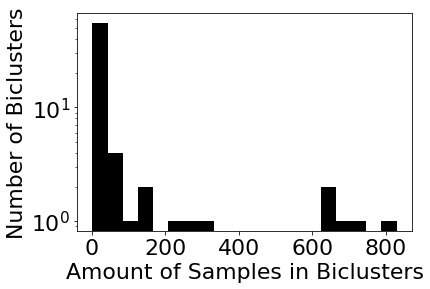
\includegraphics[width=2.5in]{figures/histogram.png}
\caption{The histogram shows the number of biclusters with a certain amount of included samples.}
\label{fig:histogram}
\end{figure}
The algorithm finds 59 biclusters in the data set with the mentioned settings.
Figure \ref{fig:histogram} shows the size distribution of the found biclusters.
It visualizes that the number of samples in a bicluster follows a power-law distribution.
Thus, it can be desirable to discard biclusters that have too few samples.
The relationship between the genes in the identified biclusters is visualized in Figure \ref{fig:cluster_gene_graph}.
In the graph, an edge is drawn if two genes occur in the same found bicluster.
Note that the resulting graph consists of two connected components.
The lower subgraph is densely connected and visualizes various connections between members of the keratin family.
This family of proteins forms the structural framework for cells that build e.g. hair.
Interestingly, keratin 14 and keratin 5 were found to interact with each other.
This emphasizes that the algorithm can infer biological processes since e.g. both genes partner in order to build the cytoskeleton of epithelial cells.
\begin{figure}[h]
\centering
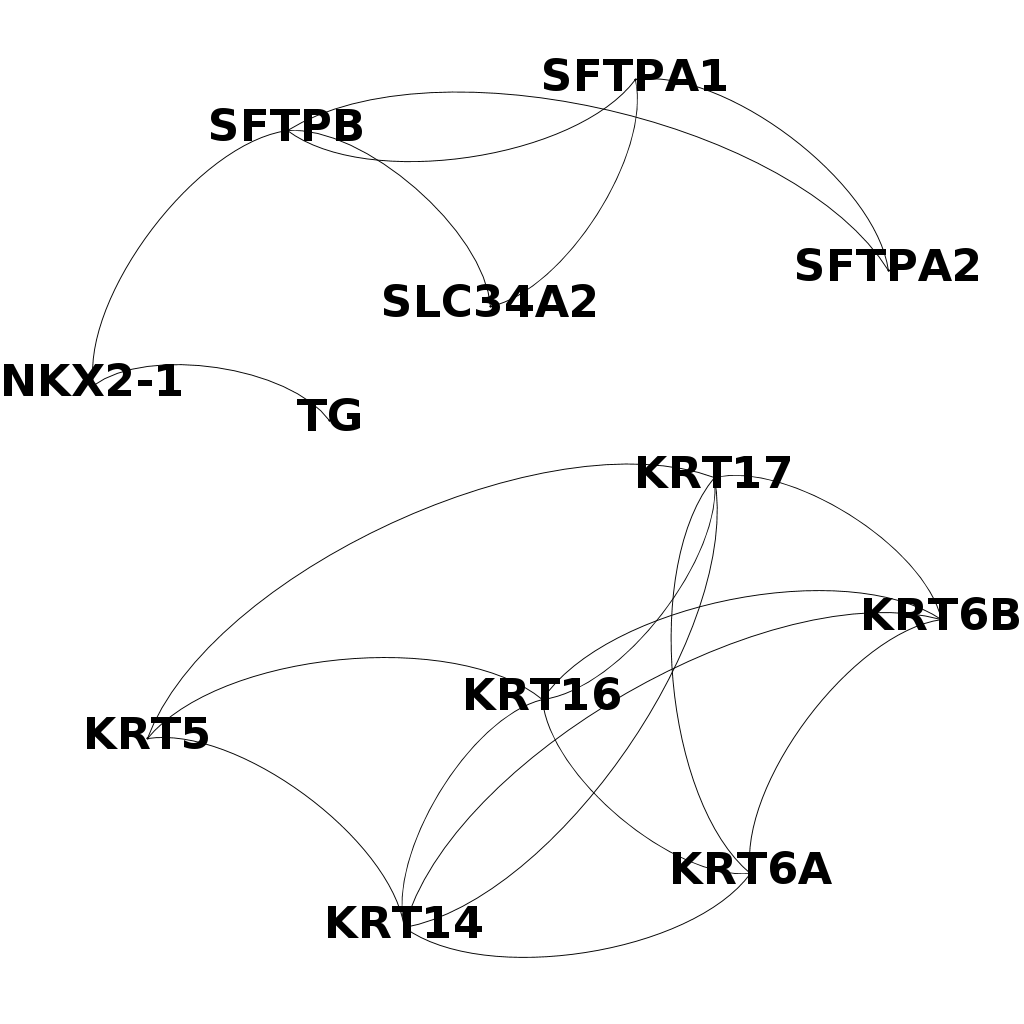
\includegraphics[width=2.5in]{figures/cluster_gene_graph.png}
\caption{The graph visualizes the interactions between clustered genes in the evaluation dataset. It shows}
\label{fig:cluster_gene_graph}
\end{figure}
We refer again to Table \ref{tab:scores} for the scores $S$ that are provided by the STRING API.
In order to evaluate which of the scores are most useful, we ran the algorithm multiple times by setting each time $s_\alpha(x, y)$ to a different $s \in S$.
To evaluate the cluster results, we calculated how many of the genes in found biclusters also interact with each other based on all scores $s \in S$.
\begin{figure}[h]
\centering
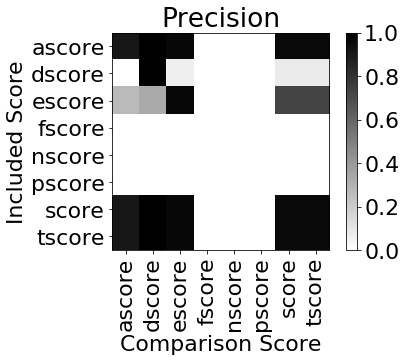
\includegraphics[width=2.5in]{figures/precision_matrix.png}
\caption{The matrix shows the precision of the algorithm based on one score compared to an other. For explanations of the scores refer to Table \ref{tab:scores}.}
\label{fig:precision}
\end{figure}
The resulting precision matrix can be found in Figure \ref{fig:precision}.
It is worth noting that the algorithm produced the best results when incorporating the coexpression score \textit{ascore}, the textmining score \textit{tscore} and the combined score \textit{score}.
We assume that the underlying information used to compute the scores is the most reliable and helpful to compute the biclusters.
The fusion score \textit{fscore}, neighborhood score \textit{nscore} and phyletic score \textit{pscore} did not yield a high precision since they were very small for the gene combinations of the preprocessed gene expression matrix.
This means that the STRING service was very unsure about whether two genes interact based on the respective information.
The reason might be that it is difficult to infer whether two genes interact with each other solely based on e.g. their nucleotide count.
The results show that while the algorithm is able to capture biological processes, its quality highly depends on the third-party data that is incorporated.
\section{Discussion}
\label{sec:discussion}
The presented approach is able to find possibly overlapping biclusters in gene expression data while incorporating biological context information.
This makes it possible to focus the search for biclusters on processes of interest only.
However, one major limitation is that the given gene expression matrix needs to be binarized so the algorithm can build an unweighted, undirected graph from that.
This makes it necessary to discard information about the exact expression levels of genes.
As described in Section \ref{sec:algorithm}, the matrix could for example be binarized by setting all cells to one that have a higher value than $\tau_e$.
This would limit the algorithm to only find biclusters of over-expressed genes.
It might also be desirable to find biclusters of over- and under-expressed genes at the same time.
For this case, we suggest to vary the criterion when a cell is set to one among different genes.
An other limitation is that the algorithm returns multiple biclusters of various sizes.
We would expect it to return the biclusters clipped and sorted by some evaluation criterion.
This metric, like the Silhouette coefficient \citep{Silhouette87} for single-mode clustering, should measure the coherence of a bicluster compared to the distance to the nearest neighboring bicluster.
The approach should therefore return biclusters of a given quality only.
\section{Conclusion}
\label{sec:conclusion}
In this work, we proposed an algorithm that finds overlapping biclusters in gene expression data while incorporating biological context information.
We showed that the detected biclusters correspond to distinct biological processes.
This enables the user to focus the bicluster detection to certain biological domains only by adjusting the third-party information that is used.
Due to the dependence on third-party information, the quality of the findings is directly influenced by the quality of the third-party data.
We thus conclude that advances in obtaining and processing biological data will also increase the performance of our algorithm.
\bibliographystyle{plainnat}
\bibliography{bibliography}
\end{document}
